%%%%%%%%%%%%%%%%%%%%%%%%%%%%%%%%%%%%%%%%%%%%%%%%%%%%%%%%
%GRASS PROMOTION FLYER                                 %
%(c) 2007 GRASS PROMOTION TEAM                         %
%GNU Free Documentation License                        %
%Version 1.2                                           %
%Needs leaflet.cls				       %
%www.ctan.org/tex-archive/macros/latex/contrib/leaflet/%
%%%%%%%%%%%%%%%%%%%%%%%%%%%%%%%%%%%%%%%%%%%%%%%%%%%%%%%%

%Sometimes printing engines need the 2nd side upside down
%in this case, use tumble (which is default) instead of notumble
%If this causes problems, use notumble
%If you need a foldmark, delete nofoldmark
\documentclass[notumble,a4paper,10pt,nofoldmark]{leaflet}
\usepackage{helvet,courier,xcolor}

% Set Helvetica as the default font
\renewcommand*\familydefault\sfdefault
% Let LaTeX knows that pictures are found in ./pix
\graphicspath{{pix/}}

% Setting up things for the captions
\usepackage{caption}[2004/07/16]
\captionsetup{%
  font={small,it},%
  labelformat=empty,% Leaves out label: ``Figure 1''
  labelsep=none,%
  aboveskip=0pt%
}
% Defining a new 'figure' environment for the document
\newenvironment{myfig}[1][0pt plus 1.5ex minus .5ex]{\par\vspace*{#1}\begin{minipage}{\textwidth}\centering}{\end{minipage}}

% Defining the GRASS homepage
\newcommand{\GRASSurl}{\url{http://grass.osgeo.org}}

% Define a color for the URIs
\definecolor{darkblue}{RGB}{0,0,88}

\usepackage{hyperref}
% Setting up some document info
\hypersetup{%
  colorlinks=true,%
  urlcolor=darkblue,% Redefine this color to change URIs color
  pdfauthor={The GRASS Community},%
  pdftitle={GRASS GIS: Efficiency through Freedom \& Transparency},%
  pdfsubject={GRASS Promotion Flyer},%
  breaklinks=true,%
  plainpages=false%
}

% Title page stuff
\title{\textbf{\huge GRASS GIS}\\%
\textsl{Efficiency through Freedom \& Transparency}}
\author{The GRASS Community}
\date{
\includegraphics[width=\textwidth]{grasslogo_vector}\\[2ex]
\large\GRASSurl}

\begin{document}

\maketitle
\thispagestyle{empty}% Necessary to leave out the page number on the first page

\newpage

\section{What is GRASS}

GRASS GIS (Geographic Resources Analysis Support System) is Free and Open Source Software for performing spatial analysis. It consists of \textbf{more than 400 modules for processing vector (2D/3D), raster, voxel and temporal data (4D)}. Many interfaces to other programs in related domains like geostatistics, databases, map web services and even other GIS software exist. It is the oldest and largest Free and Open Source GIS. It can serve as a Desktop GIS and as the backbone of a complete GIS infrastructure.

\section{Where is GRASS used}

GRASS GIS is used in scientific applications, commercial settings and by public authorities all over the world. GRASS GIS has shown strong potential for solving geospatial problems in numerous situations world-wide.

\section{History}

GRASS GIS was originally developed in the early 1980's by the US Army Construction Engineering Research Laboratories (USA-CERL) and was published as public domain software. When the USA-CERL withdrew from GRASS GIS development, an international developer team assumed responsibility for the task. Since 1999, GRASS GIS has been published as free software under the terms of the GNU General Public Licence. Several people during years contributed to improve the software, they helped to add new functionality, speedup existing modules, make \textbf{GRASS GIS easier, more useful and powerful to everybody}. \newline

\begin{myfig}
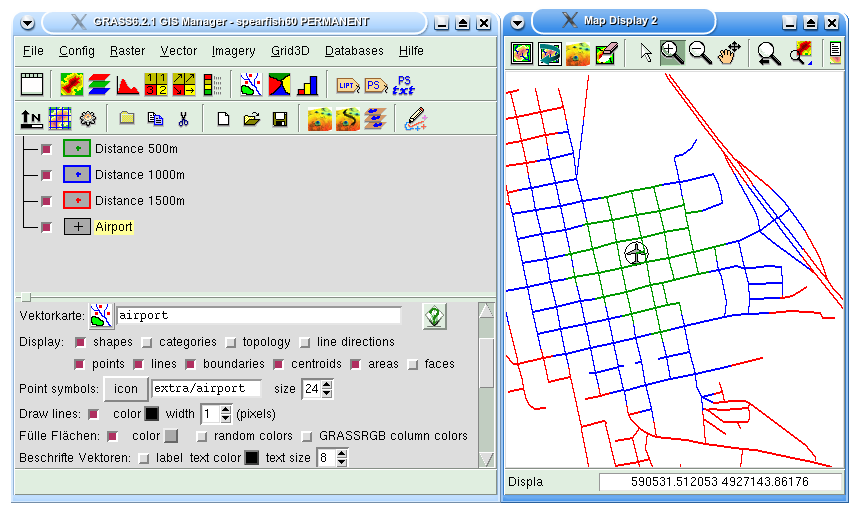
\includegraphics[width=0.8\textwidth]{isodist}
\captionof{figure}{Default GUI configuration showing GRASS network analysis capabilites}
\end{myfig}


\section{Free and Open Source Philosophy}

The Free and Open Source philosophy lets the user see the source code and structure of the program, which offers great transparency. Users can extend the program for their own needs. Immediate source code peer review increases the quality. With the help of the extension manager, new modules can be created without GRASS GIS package source code.

\section{Technical Data Sheet}

\subsection{License}

GNU General Public License (Free Software Foundation)

\subsection{Supported platforms}

GRASS runs on nearly all platforms. It supports GNU/Linux, Posix compliant Unix Systems, MS-Windows and MacOS X.

\subsection{Design}

\begin{itemize}
\item Modular commands
\item Consists of more than 400 modules
\end{itemize}

\subsection{Programming languages}

\begin{itemize}
\item ANSI C
\item GRASS-SWIG interface
\item Python API, scripting library and GUI
\end{itemize}

\subsection{Data management capabilities}

\begin{itemize}
\item Raster / Vector / Voxel data processing
\item 2D / 3D Raster / Vector modeling
\item Image manipulation
\item Vector topology / Network analysis
\item Geostatistics (Interface to R)
\item Temporal dataset
\item WPS interface
\end{itemize}

\begin{myfig}[1ex]
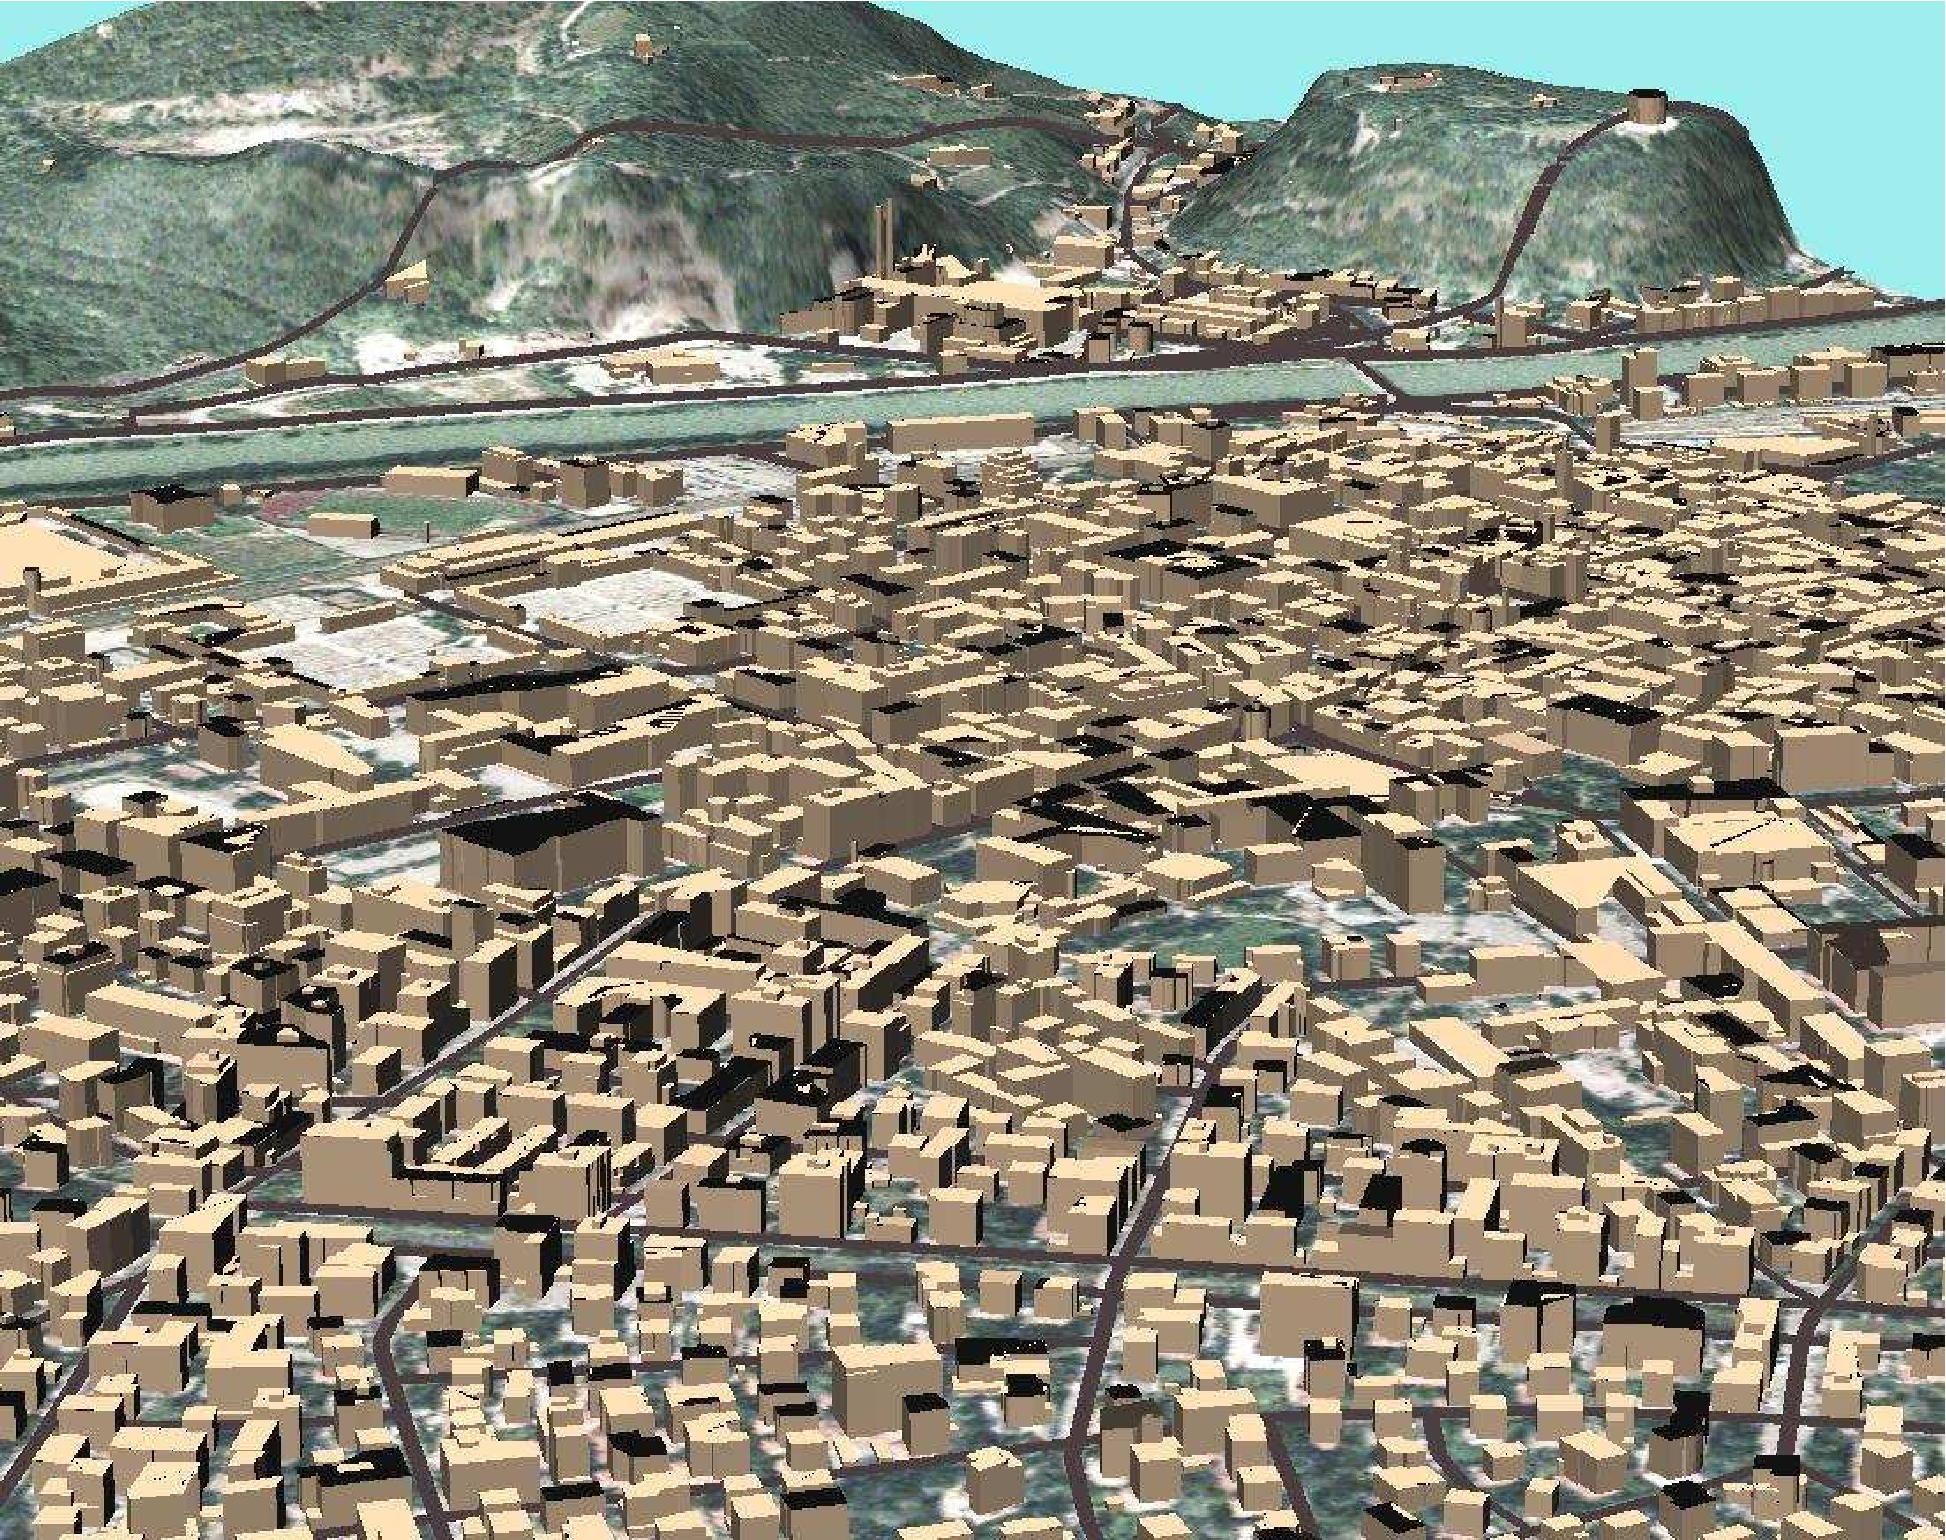
\includegraphics[width=0.7\textwidth]{trento3d}
\captionof{figure}{A flyby of the city of Trento, Italy}
\end{myfig}

\section{Supported file formats}

GRASS supports nearly all common GIS file formats through the use of the GDAL/OGR library. It also supports the Open GIS Consortium's Simple Features.

\subsection{Vector file formats}
ASCII, ARC/INFO ungenerate, ARC/INFO E00, Arc\-View SHAPE, BIL, DLG (U.S.), DXF, DXF3D, GMT, GPS-ASCII USGS-DEM, IDRISI, MOSS, MapInfo MIF, PostGIS, TIGER, VRML, \dots

\subsection{Raster file formats}
ASCII, ARC/GRID, E00, GIF, GMT, TIF, PNG, Vis5D, SURFER (.grd),\dots
\begin{myfig}[1.ex]
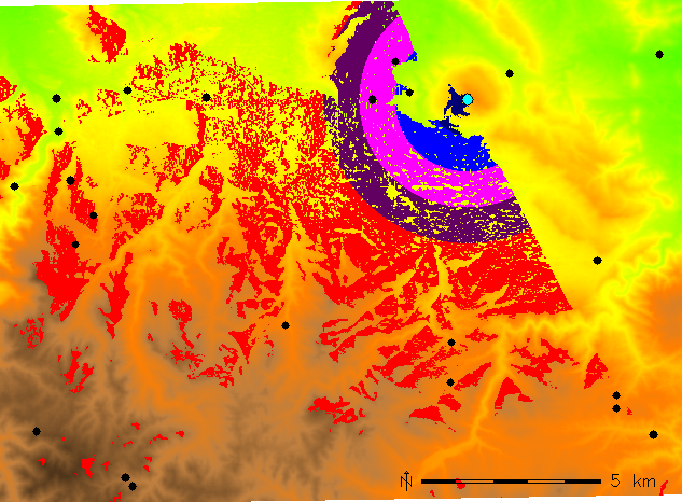
\includegraphics[width=0.7\textwidth]{visibility}
\captionof{figure}{Viewshed analysis performed with GRASS}
\end{myfig}

\subsection{Image file formats}

CEOS (SAR, SRTM, LANDSAT7 etc.), ERDAS LAN / IMG, HDF, LANDSAT TM/MSS, NHAP aerial photos, SAR, SPOT, MODIS \dots
% \begin{myfig}[1.5ex]
% 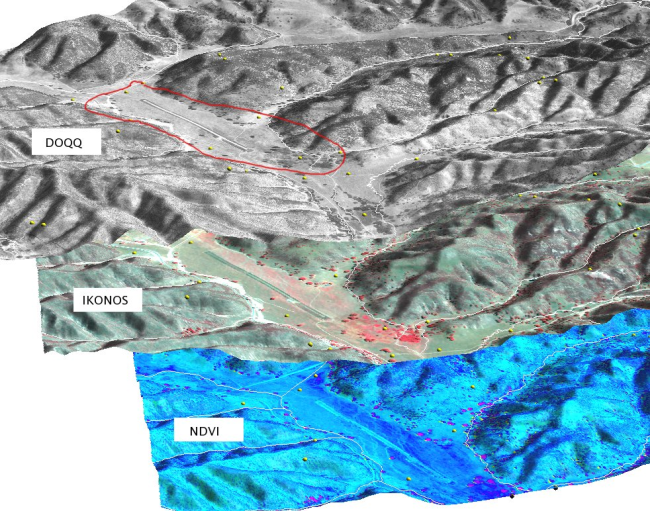
\includegraphics[width=0.7\textwidth]{ndvi}
% \captionof{figure}{Image processing options in GRASS}
% \end{myfig}
\begin{myfig}
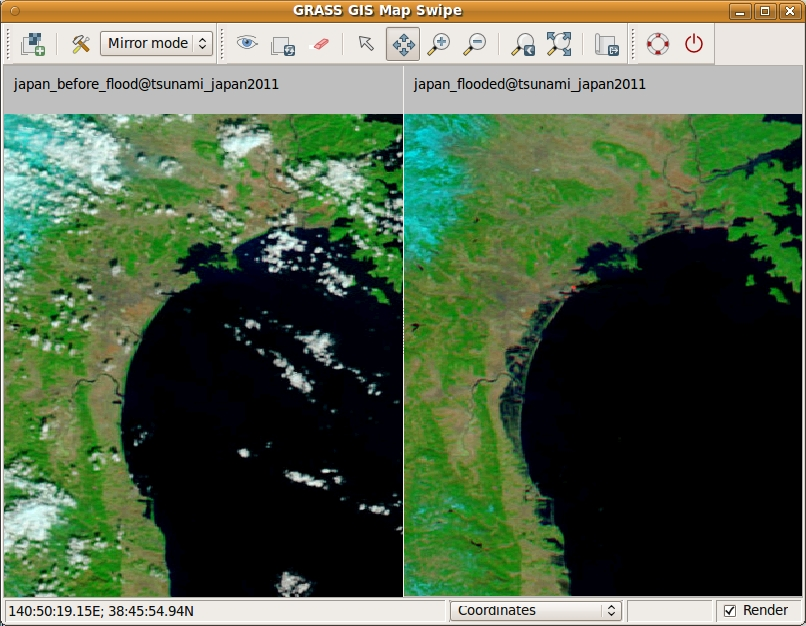
\includegraphics[width=0.7\textwidth]{mapswipe}
\captionof{figure}{MapSwipe tool showing differences before and after Japan Tsunami 2011}
\end{myfig}

\subsection{Database support}

\begin{itemize}
\item SQLite
\item PostgreSQL / PostGIS
\item MySQL
\item ODBC
\item DBF
\end{itemize}

\subsection{Output}

\begin{itemize}
\item Mapping modules (animation, cartographic \dots)
\item NVIZ for visualization of 2.5D and 3D data (creation of animations \& flybys)
%\item{GMT export}
%item{VRML}
\item VTK, POVray
\item Web Services
\end{itemize}

\subsection{Interoperability with other GIS-related Software}

\begin{itemize}
\item QGIS (Free geodata viewer and more)
\item R-Language (Statistics)
\item Gstat (Geostatistics)
\item UMN MapServer (Webmapping)
\end{itemize}

\section{Where to find more information}

\begin{itemize}
% \begin{flushleft}
\item{Project Website: \\\GRASSurl}
\item{GRASS Wiki: \\\url{http://grass.osgeo.org/wiki}}
% \item{GRASS Promotion Team: \\\url{malte@perlomat.de}}
\item{GRASS mailing lists: \\\url{http://grass.osgeo.org/community}}
% \end{flushleft}
\end{itemize}

\vfill
\section{OSGeo}

GRASS is a founding project of the Open Source Geospatial Foundation which has the aim to create high quality open source geospatial software. For further information visit the OSGeo homepage:
\begin{center}

\includegraphics[width=0.7\textwidth]{OSGeo_CMYK}\\
\url{http://www.osgeo.org}
\end{center}

\end{document}
